
\documentclass{lxaiproposal}
  
  
%   \usepackage[english,french]{babel}   % "babel.sty" + "french.sty"
\usepackage[english]{babel}   % "babel.sty" + "french.sty"
   
% \usepackage[english,francais]{babel} % "babel.sty"
% \usepackage{french}                  % "french.sty"
\usepackage{times}			% ajout times le 30 mai 2003
 
\usepackage{epsfig}
\usepackage{graphicx}
\usepackage{amsmath}
\usepackage{amssymb}
\usepackage{booktabs}
\usepackage{multirow}
\usepackage{pifont}
\usepackage{caption}
\usepackage{subcaption}
\usepackage{jm}


\usepackage{array}
\usepackage{color}
\usepackage{colortbl}

\usepackage{pifont}
\usepackage{amssymb}
\usepackage{latexsym}

\usepackage{booktabs}

%% --------------------------------------------------------------
%% FONTS CODING ?
% \usepackage[OT1]{fontenc} % Old fonts
% \usepackage[T1]{fontenc}  % New fonts (preferred)
%% ==============================================================

\title{Qualify Exam Proposal}

\author{\coord{Yuyang}{Ma}{}}

\address{\affil{}{Department of Industrial and Systems Engineering, Lehigh University, Bethlehem, PA, United States}}

%% If all authors have the same address %%%%%%%%%%%%%%%%%%%%%%%%%%%%%%%%%%%%%%%
%                                                                             %
%   \auteur{\coord{Michel}{Dupont}{},                                         %
%           \coord{Marcel}{Dupond}{},                                         %
%           \coord{Michelle}{Durand}{},                                       %
%           \coord{Marcelle}{Durand}{}}                                       %
%                                                                             %
%   \adress{\affil{}{Laboratoire Traitement des Signaux et des Images \\      %
%     1 rue de la Science, BP 00000, 99999 Nouvelleville Cedex 00, France}}   %
%                                                                             %
%                                                                             %
%%%%%%%%%%%%%%%%%%%%%%%%%%%%%%%%%%%%%%%%%%%%%%%%%%%%%%%%%%%%%%%%%%%%%%%%%%%%%%%

\email{yuyang.ma@lehigh.edu}

\englishabstract{This proposal focuses on the extension of the paper \cite{dukkanci2023drones} topic on a post-disaster delivery problem called the relief distribution problem using drones under uncertainty. In the paper, the authors proposed to use unmanned aerial vehicles (UAVs) as the primary delivery methods. They considered uncertainties in victims' demand and road conditions. The problem was formulated as a two-stage stochastic programming model to minimize unmet demand, solved using a scenario decomposition algorithm (SDA). In my report, I propose to incorporate uncertain weather conditions into the current formulation. I will also consider more constraints for large drone usage. Additionally, I will reformulate the model using sample average approximation (SAA) and solve it using the Benders decomposition algorithm. A comparison between SDA and the Benders decomposition algorithm will be conducted. Finally, I will analyze the value of stochastic modeling and the expected value of perfect information. This proposal aims to: 1. Provide committee members a background of delivery with drones; 2. Briefly demonstrate the content of the paper \cite{dukkanci2023drones}; 3. State the proposed extensions of the paper and corresponding motivations.}

\begin{document}
\maketitle
\section{Background and Motivation}
\vspace*{-3mm}


As drone technology has rapidly developed, their application in various fields has been extensively studied. In the commercial delivery sector, leading organizations like UPS \cite{ups2017drone} and Amazon \cite{amazon2022drone} have utilized drones to deliver packages. Additionally, drones have demonstrated their potential in humanitarian and healthcare operations. For example, in collaboration with other organizations, DHL successfully tested the delivery of medicines using a drone to an island in Lake Victoria. Due to poor infrastructure and difficult terrain, medical supplies for the approximately 400,000 residents of Ukerewe Island in Lake Victoria were severely limited. However, thanks to the advantages of drones, such as ignoring road conditions and rapid flying speed, the delivery time was successfully reduced from six hours to 40 minutes. Emergency deliveries in such areas are no longer an impossible mission \cite{dhl2018drone}.


\section{Brief Review of the Paper \cite{dukkanci2023drones}}
\vspace*{-3mm}


Motivated by the aforementioned applications, Dukkanci et al. explored the potential of using drones to do the last-mile delivery in the post-disaster humanitarian application \cite{dukkanci2023drones}. Under the scenario of an earthquake, the victims will stay at different assembly points (gathering points). The road connections between gathering points and the distribution center of relief items may be disrupted owing to the possible debris in the area of gathering points and supply points. The UAVs can be used as the main delivery method to distribute relief items to affected people by minimizing the impact of such an incomplete road network.

In the paper, the authors divide all locations into 3 categories: gathering points, distribution centers (depot), and launch points. The gathering points are the locations where victims stay and wait for the relief items. The depot is the location where the relief items are stored. The launch points are the locations where the trucks can reach out after the earthquake. The authors proposed a two-echelon delivery system, which consists of two different kinds of UAVs, large drones and small drones. The large drones, which have a longer flight range, deliver the relief items directly from the depot to the gathering point. For small drones, depending on the distance between the depot and the gathering points, they can either deliver the relief items directly from the depot to the gathering points, or from the launch points to the gathering points after trucks carrying drones and demanding relief items to the launch points.

As for the aspect of uncertainties, Dukkanci et al. considered two types of uncertainties: the uncertainty in victims' demand and road conditions. They formulated the problem as a two-stage stochastic programming model to minimize the unmet demand, constrained by drones' payload limit and battery capacity. They also stipulated that all delivery activities must be completed within a specified time window. The model was solved using a scenario decomposition algorithm (SDA), which was proposed by S. Ahmed \cite{ahmed2013SDA}. The authors conducted a real-life application to show the effectiveness of the proposed formulation and the SDA algorithm.


\section{Proposed Extensions}
\vspace*{-3mm}


As for the content of my qualifying exam, I propose to extend the work of Dukkanci et al. in the following aspects:
\begin{enumerate}
    \item[1.] Considering uncertain weather conditions, which may affect the delivery time of drones;
    \item[2.] Incorporating more constraints for large drones;
    \item[3.] Reformulating the model using SAA, solving it with the Benders decomposition algorithm, and comparing the performance of SDA and the Benders decomposition algorithm;
    \item[4.] Analyzing the value of stochastic modeling and the expected value of perfect information.
\end{enumerate}
More detailed explanations are provided in the following subsections:


\subsection{Uncertain Weather Conditions}
\vspace*{-1mm}
Unlike traditional delivery methods like trucks, one of the significant challenges for drones is the weather conditions. The weather conditions like wind speed, temperature, and humidity may affect the flight conditions and the energy consumption of drones.


In the paper \cite{dukkanci2023drones}, the authors neglect the weather conditions for simplicity. The calculation of the range for small drones is based on Dukkanci's study \cite{dukkanci2021minimizing}, where the drone range depends on the energy consumption formula by Stolaroff et al. \cite{stolaroff2018energy}, estimated using the power consumption formula developed by Zeng et al. \cite{zeng2019energy}. The range $R(v)$ (in m) of a drone traveling at a constant speed $v$ (in m/s) is expressed as follows:
\begin{equation}
    R(v) = \frac{\Theta}{\frac{\mu_1}{v} + \mu_2 v + \frac{\mu_3}{v^2} + \mu_4 v^2}, \label{eq:range_formula}
\end{equation}
where $\Theta, \mu_1, \mu_2, \mu_3$ and $\mu_4$ are constants.


As one of the proposed extensions, the uncertain wind speed will be incorporated into the stochastic programming model proposed by Dukkanci et al. The wind speed will be modeled as a random variable under an estimated distribution. In figure \ref*{fig:wind_speed}, the effect of wind speed on the flight time of drones is shown, where the \textit{air speed} is the speed of the drone, and \textit{ground speed} is the resulting speed of the drone after considering the wind speed \cite{cheng2024robust}.
\begin{figure} [h!]
    \centering
    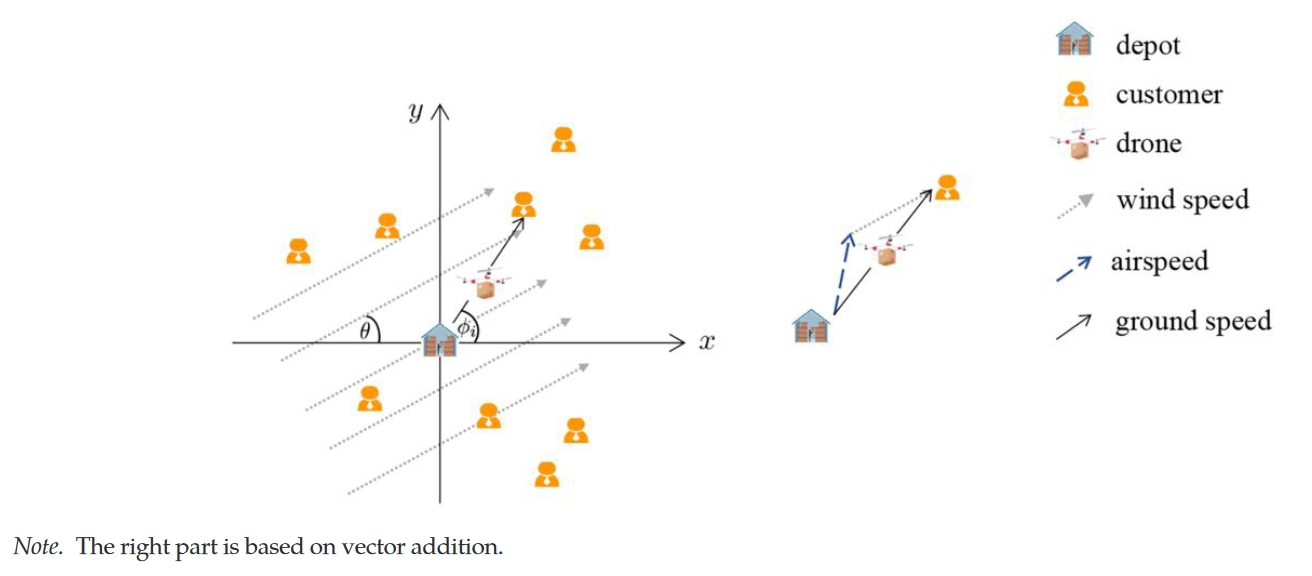
\includegraphics[width=1\linewidth]{figure_windspeed.png}
    \caption{Calculating Flight Times \cite{cheng2024robust}}
    \label{fig:wind_speed}
\end{figure}
The wind speed will affect the speed and further affect the flight time of drones, assignment of drones, and even locations of launch points, and depots.


\subsection{Constraints for Large Drones}
\vspace*{-2mm}
As one of two delivery methods considered in the paper \cite{dukkanci2023drones}, the large drone plays an important role when optimizing the delivery system. Assumptions on its property can significantly affect the construction of the constraints. However, Dukkanci et al. assumed that large drones are not range-limited and the payload weight has no impact on their flight ranges, which is too ideal to be true. In the proposed extension, I will incorporate more constraints for large drones. For example, the limited range will be considered for large drones, which means the large drones also have a limited speed and the flight time will be affected by the wind speed.


\subsection{Benders Decomposition}
\vspace*{-2mm}
Benders decomposition is a well-known algorithm for solving two-stage stochastic programming problems. It decomposes the original problem into a master problem and a subproblem. A detailed recap of Benders decomposition will be conducted in the exam report. The Benders decomposition algorithm has been widely used in many areas, like transportation, energy, and finance.

Note that in the modified stochastic programming model, I will work on a pure integer programming problem, meaning the dual cannot be well-defined. Some modifications to the traditional Benders decomposition need to be implemented. One famous modification to Benders decomposition to solve stochastic integer programming has been conducted by Laporte et al. \cite{laporte1993integer}. In the proposed extension, I will reformulate the existing stochastic programming model using SAA and solve it using the Benders decomposition algorithm. A comparison between results solved by SDA and the Benders decomposition algorithm will be conducted.


\subsection{Analysis of the Value of Stochastic Solution and the Expected Value of Perfect Information}
\vspace*{-2mm}
As two important metrics in stochastic programming and decision analysis, the loss by not considering the random variations is the difference between this and the stochastic model is the \textit{value of the stochastic solution (VSS)}, and the difference between the expected value of a decision made with perfect information and the expected value of a decision made under uncertainty is called the \textit{expected value of perfect information (EVPI)}. As stated in the book by Birge et al., "\textit{EVPI} measures the value of knowing the future with certainty while \textit{VSS} assesses the value of knowing and using distributions on future outcomes \cite{birge2011introduction}." In the proposed extension, I will analyze the value of stochastic modeling and the expected value of perfect information. The results will provide insights into the value of stochastic modeling and the potential benefits of collecting more information.


\section{Discussion}
\vspace*{-3mm}


After conducting the proposed extensions, compared to the formulation proposed in the original paper \cite{dukkanci2023drones}, the new formulation is more realistic and can better reflect the real-world situation. The incorporation of uncertain weather conditions will make the model more robust and reliable. The constraints for large drones will make the model more practical and can provide more insights into the usage of large drones. However, because of more sophisticated constraints, the model may become more complex and harder to solve. Compared to the existing formulation, the optimal value of the new formulation is expected to be larger, and the new formulation is expected to be solved in a longer time.



% Please add the following required packages to your document preamble:
% \begin{table}[h!]
% \centering
% \caption{A typical table.}
% \label{tab:my-table}
% \begin{tabular}{@{}ccccc@{}}
% \toprule
% \textbf{Items/Cols} & \textbf{Col 1} & \textbf{Col 2} & \textbf{Col 3} & \textbf{Col 4} \\ \midrule
% \textbf{Item 1}     & Value          & Value          & Value          & Value          \\
% \textbf{Item 2}     & Value          & Value          & Value          & Value          \\
% \textbf{Item 3}     & Value          & Value          & Value          & Value          \\ \bottomrule
% \end{tabular}
% \end{table}

 %\begin{figure} [h!]
 %    \centering
 %    \includegraphics[width=1\linewidth]{images/fig1.png}
 %  \caption{A typical figure.}
 %    \label{fig:my-fig}
 %    \end{figure}

\bibliographystyle{ieee_fullname}
\bibliography{references}

%\begin{thebibliography}{99}
%\end{thebibliography}

\end{document}
